\documentclass{article}
\usepackage{iclr2026_conference,times}
\usepackage{amsmath,amssymb,amsthm,booktabs}
\usepackage{graphicx}
\usepackage{array}
\usepackage{hyperref}
\usepackage{url}

\title{Semantic Force Closure: Task-Legal Contact Certificates for Robotic Grasping}
\author{Anonymous Authors}

\newtheorem{definition}{Definition}
\newtheorem{proposition}{Proposition}
\newtheorem{claim}{Claim}
\newcommand{\sfc}{\mathrm{SFC}}

\begin{document}
\maketitle

\paragraph{Submission-hardening version: v3 final full-scale.}
This revision expands the original 720-trial note into a full-scale synthetic certificate study with 75,520 policy/certificate rows over 12,032 contact cases, seven experiment families, risk-aware and abstaining semantic certificates, post-hoc witness search, friction/cone sensitivity, ablations, negative controls, and a counterexample library. The final claim is deliberately scoped: SFC changes the certificate witness and exposes task-illegal geometric force closure; it does not solve semantic perception, tactile estimation, dynamics, compliance, or real-robot grasping.

\begin{abstract}
Robotic grasping often treats semantics as a pre-filter or post-filter around a geometric force-closure test. That separation is unsafe for task-oriented manipulation: a grasp can be geometrically force closed because its certificate touches a blade, rim, screen, nozzle, stem, hot base, needle, or other role that the task forbids. We introduce Semantic Force Closure (SFC), a task-conditioned certificate that deletes task-forbidden contact-role wrench generators before checking whether the origin remains in the convex hull of the surviving generators. In a 75,520-row planar certificate study over 12,032 contact cases, ordinary geometric force closure accepts every Family A contact cloud, but the selected geometric witness is task-legal in 0.0\% of those cases under the trap-heavy witness selection protocol. Oracle SFC finds a legal witness in 46.3\%, semantic-only acceptance is unsafe in 53.7\%, single-witness post-hoc filtering misses every legal SFC witness in the main family, and soft semantic penalties accept unsafe witnesses in 100.0\%. Under 10\% calibrated role-label error, observed SFC produces 28.3\% unsafe certificates, while a risk-aware thresholded variant records 0.0\% unsafe certificates in the same slice at the cost of changed coverage. The result is not that SFC certifies more grasps; it certifies fewer but legal grasps, exposes when a geometric witness is illegal, and makes role-label uncertainty a first-class safety variable.
\end{abstract}

\section{Introduction}

Task-oriented grasping has two obligations that are often separated. The grasp must be mechanically stable, and it must touch the object in task-legal places. Classical force closure addresses mechanical stability with wrench geometry. Semantic grasping, affordance grounding, task-conditioned datasets, contact semantic maps, and recent foundation-model grasp planners address task meaning by ranking, masking, or describing contacts \citep{lit001,lit003,lit004,lit011,lit018,lit055}. The problem is that these two modules do not commute. A force-closure certificate found over all contacts may rely on a forbidden role. Removing that role after the fact can destroy the wrench balance. Conversely, a geometric witness can be illegal even when another legal witness exists.

This paper studies the certificate-ordering version of that problem. Semantic Force Closure deletes every wrench generator attached to a task-forbidden contact role before solving the convex-hull force-closure feasibility problem. The mechanism is small, but the ordering matters: semantics constrain the witness, not only the candidate score.

The simplest example is a knife pass. A grasp can be geometrically stable because it touches both handle and blade. For a handoff task, blade contacts are illegal even if they make the wrench hull large. A post-hoc filter that rejects the chosen geometric witness may miss an alternative handle-only witness; a semantic-only filter that checks for handle contacts may accept a grasp whose handle contacts cannot balance wrench space. SFC asks the direct question: after deleting blade and edge generators, does the surviving handle/pommel generator set still certify force closure?

The v2 paper already showed this effect in 720 deterministic trials and found a 34.6\% geometric optimism gap. It also showed that role-label noise can create unsafe false certificates. The present v3 version scales the evidence, adds stronger baselines and negative controls, and makes the failure cases central rather than peripheral. The study remains synthetic and planar. That limitation is intentional: we want to isolate the certificate ordering before claiming any perception or hardware result.

\paragraph{Contributions.}
The paper makes four contributions:

\begin{itemize}
\item A certificate-level definition of Semantic Force Closure in which task semantics delete wrench generators before convex-hull feasibility.
\item A full-scale synthetic benchmark with 75,520 policy/certificate rows over 12,032 contact cases spanning task geometry, semantic noise, witness ordering, friction/cone perturbations, ablations, negative controls, and counterexamples.
\item Evidence that ordinary geometric FC, semantic-only acceptance, soft penalties, and single-witness post-hoc filtering can all accept or miss the wrong witnesses under task-role constraints.
\item An explicit uncertainty boundary: noisy observed SFC can be unsafe, while risk-aware and abstaining variants trade coverage for safety under role ambiguity.
\end{itemize}

\section{Related Work}

\paragraph{Force closure and grasp quality.}
Classical grasp analysis asks whether contact wrench cones can balance arbitrary external wrenches. Convex hull, grasp matrix, friction cone, and LMI formulations are standard tools \citep{lit007,lit009,lit015}. This paper does not claim new force-closure mathematics. It reuses the convex-hull view and changes which generators are allowed to enter the certificate.

\paragraph{Semantic and affordance-aware grasping.}
Semantic grasping and affordance methods condition grasps on object parts, tasks, language, and functional constraints \citep{lit003,lit004,lit008,lit011,lit012,lit043,lit055}. These methods are increasingly strong at proposing task-appropriate contacts. SFC is complementary: after a proposal and role labels exist, the certificate must be computed over task-legal generators only. A semantic ranking can propose handle contacts; SFC checks whether those contacts carry the wrench witness.

\paragraph{Contact semantic maps and dexterous datasets.}
Large grasp datasets and contact semantic maps improve the representation of hand-object contact \citep{lit001,lit018,lit057}. They make it natural to know whether a contact touches a handle, blade, rim, screen, nozzle, or other role. SFC asks that these role labels be used inside the certificate. Dataset scale does not remove the need to audit the witness.

\paragraph{Tactile verification and uncertainty.}
Tactile sensing and friction estimation can help validate contact states and slip boundaries \citep{lit048}. The present paper does not implement tactile estimation. Instead it uses synthetic label noise to show why a deployed SFC system must propagate role uncertainty rather than deleting contacts from point estimates.

\section{Semantic Force Closure}

Let a contact cloud be \(C=\{c_i\}_{i=1}^{n}\). Each contact has a role \(r_i\), a point \(p_i\), a friction parameter \(\mu_i\), and a set of linearized friction-cone wrench generators \(W_i=\{w_{ij}\}_{j=1}^{m_i}\subset\mathbb{R}^3\). A task \(\tau\) supplies a set of allowed roles \(A(\tau)\). Examples are handle, body, edge, base, and stem-lower roles; examples of forbidden roles are blade, edge, rim, screen, nozzle, hot base, needle, and petal.

\begin{definition}[Geometric force closure]
A contact cloud is geometrically force closed under the local linearized model if the origin lies in the convex hull of all available wrench generators:
\[
0\in \operatorname{conv}\left(\bigcup_{i=1}^{n} W_i\right).
\]
\end{definition}

\begin{definition}[Semantic Force Closure]
A contact cloud is semantically force closed for task \(\tau\) if the origin lies in the convex hull after deleting all generators attached to forbidden roles:
\[
0\in \operatorname{conv}\left(\bigcup_{i:r_i\in A(\tau)} W_i\right).
\]
\end{definition}

Equivalently, SFC is feasible when there are nonnegative coefficients \(\lambda_{ij}\) such that
\[
\sum_{i:r_i\in A(\tau)} \sum_j \lambda_{ij} w_{ij}=0,
\qquad
\sum_{i:r_i\in A(\tau)} \sum_j \lambda_{ij}=1.
\]
The certificate witness is the set of contacts with nonzero coefficient. The witness is not an incidental detail. If it contains a forbidden role, the certificate is mechanically valid but task-illegal.

\begin{proposition}[Subset monotonicity]
In the same wrench model, SFC implies geometric force closure.
\end{proposition}

\begin{proof}
The SFC generator set is a subset of the geometric generator set. If the origin lies in the convex hull of the subset, it also lies in the convex hull of the superset.
\end{proof}

\begin{proposition}[The converse fails]
Geometric force closure does not imply SFC.
\end{proposition}

\begin{proof}
Choose a contact cloud whose only force-closure witness requires a forbidden role. The origin lies in the convex hull of all generators but not in the convex hull of the surviving allowed generators. The generated counterexample library contains such cases, including knife-pass contact clouds where the all-contact witness uses blade/edge roles while the handle/pommel subset is rank-poor.
\end{proof}

\paragraph{LP certificate.}
The implementation solves a bounded linear program. Given a generator matrix \(G\in\mathbb{R}^{3\times m}\), it maximizes the minimum witness weight \(t\):
\[
\max_{\lambda,t} t
\quad\text{s.t.}\quad
G\lambda=0,\quad
\mathbf{1}^{\top}\lambda=1,\quad
\lambda_k\ge t,\quad
\lambda_k\ge0,\quad t\ge0.
\]
The quality score is the optimized \(t\). A positive value certifies that the origin is represented by a nonnegative convex combination with nontrivial support. The same LP is used for geometric FC, oracle SFC, observed SFC, risk-aware SFC, and post-hoc witness searches; only the generator set changes.

\section{Methods Compared}

\paragraph{Geometric FC.}
Geometric FC checks all contacts regardless of role. It is a mechanical certificate but not a task-legal certificate unless its active witness contacts are all allowed. In the main Family A protocol, it accepts 100.0\% of contact clouds but its active witness is task-legal in 0.0\%.

\paragraph{Oracle SFC.}
Oracle SFC uses the true role labels and deletes forbidden generators before the LP. It is the mechanism reference. It is not a perception system and not a deployable guarantee when labels are uncertain.

\paragraph{Observed SFC.}
Observed SFC deletes contacts using corrupted observed role labels. It can accept true-forbidden contacts mislabeled as allowed. This is the main safety attack.

\paragraph{Risk-aware SFC.}
Risk-aware SFC keeps observed-allowed contacts only when their role confidence exceeds a threshold. It is a simple uncertainty-aware certificate. It can reduce unsafe certificates but may miss true legal witnesses.

\paragraph{Abstaining SFC.}
Abstaining SFC refuses to certify when low-confidence allowed labels are present. It is conservative and is evaluated as a coverage/safety tradeoff.

\paragraph{Semantic-only acceptance.}
Semantic-only acceptance checks whether enough allowed contacts exist, without checking wrench balance. It is intentionally weak; it models systems that treat semantics as sufficient.

\paragraph{Post-hoc filtering.}
Single-witness post-hoc filtering runs geometric FC first, then rejects the chosen witness if it uses forbidden contacts. Top-\(k\) post-hoc filtering searches multiple geometric witnesses. This probes noncommutativity: filtering a witness after the geometric certificate is not equivalent to computing the certificate after deletion.

\paragraph{Soft semantic penalties.}
Soft-penalty FC allows forbidden contacts but subtracts a penalty from witnesses that use them. This models treating semantics as a cost rather than a hard certificate constraint.

\section{Full-Scale Experiment Design}

The v3 suite contains seven families. Each family writes rows to CSV, summaries to CSV, tables to \LaTeX, and figures to PDF/PNG. The run is deterministic with seed 24024 and records zero plot failures.

\paragraph{Family A: task and geometry sweep.}
Family A spans ten task templates: knife pass, mug serve, phone pickup, spray bottle use, apple pick, scissors pass, syringe handoff, pan carry, tablet pickup, and flower cut. It varies contact density, trap strength, and friction band. It produces 16,200 method rows over 3,240 contact cases.

\paragraph{Family B: semantic noise and uncertainty.}
Family B corrupts observed role labels at 0, 2, 5, 10, 20, 30, and 40\% error. It tests calibrated, overconfident, underconfident, and adversarial confidence models with risk thresholds 0.55, 0.70, and 0.85. It produces 40,320 rows over 5,040 cases.

\paragraph{Family C: witness ordering.}
Family C evaluates top-\(k\) post-hoc filtering with budgets 1, 2, 4, 8, and 16. It tests whether searching more geometric witnesses can recover legal SFC witnesses. It produces 4,320 rows over 1,440 cases.

\paragraph{Family D: friction and model perturbation.}
Family D varies friction bands and cone facets, and perturbs contact positions and friction. It produces 3,840 rows over 768 cases.

\paragraph{Family E: ablations.}
Family E isolates deletion ordering, post-hoc filtering, semantic-only acceptance, soft penalties, noisy-role deletion, and auditless geometric declarations. It produces 2,520 rows over 360 cases.

\paragraph{Family F: negative controls.}
Family F includes all roles allowed, no roles allowed, random roles, geometrically infeasible clouds, no forbidden-contact advantage, and ordinary controls. It produces 1,920 rows over 384 cases.

\paragraph{Family G: counterexample library.}
Family G records explicit geometric-not-SFC, semantic-only-not-SFC, post-hoc-miss, unsafe observed-SFC, and no-legal-witness cases. It produces 6,400 rows over 800 cases.

\section{Results}

\subsection{Main Certificate Gap}

Table~\ref{tab:main} reports the main Family A result. Ordinary geometric FC accepts every contact cloud because the full role set is mechanically rich. That is exactly the failure mode: its active witness is task-legal in 0.0\% of cases under the trap-heavy witness selection protocol. Oracle SFC accepts 46.3\% of cases. The remaining 53.7\% are not failures of SFC; they are cases where no legal allowed-role witness exists under the local model.

\begin{table}[t]
\centering
\caption{Family A full-scale benchmark. ``Accept'' means the method returns a certificate or acceptance decision. ``True legal'' means the returned certificate is legal under true task roles.}
\label{tab:main}
\begin{tabular}{lrrrr}
\toprule
Method & Accept & True legal & Unsafe & Missed true \\
\midrule
geometric\_fc & 100.0 & 0.0 & 100.0 & 46.3 \\
oracle\_sfc & 46.3 & 46.3 & 0.0 & 0.0 \\
semantic\_only & 100.0 & 46.3 & 53.7 & 0.0 \\
posthoc\_single & 0.0 & 0.0 & 0.0 & 46.3 \\
soft\_penalty\_fc & 100.0 & 0.0 & 100.0 & 46.3 \\
\bottomrule
\end{tabular}

\end{table}

Semantic-only acceptance accepts 100.0\% but is true-legal only when oracle SFC exists, so it is unsafe in 53.7\%. Single-witness post-hoc filtering accepts 0.0\%; it rejects the geometric witness whenever it uses forbidden roles and does not search the allowed subset. Soft penalties accept 100.0\% while remaining true-legal in 0.0\%, showing that a penalty is not a certificate.

\begin{figure}[t]
\centering
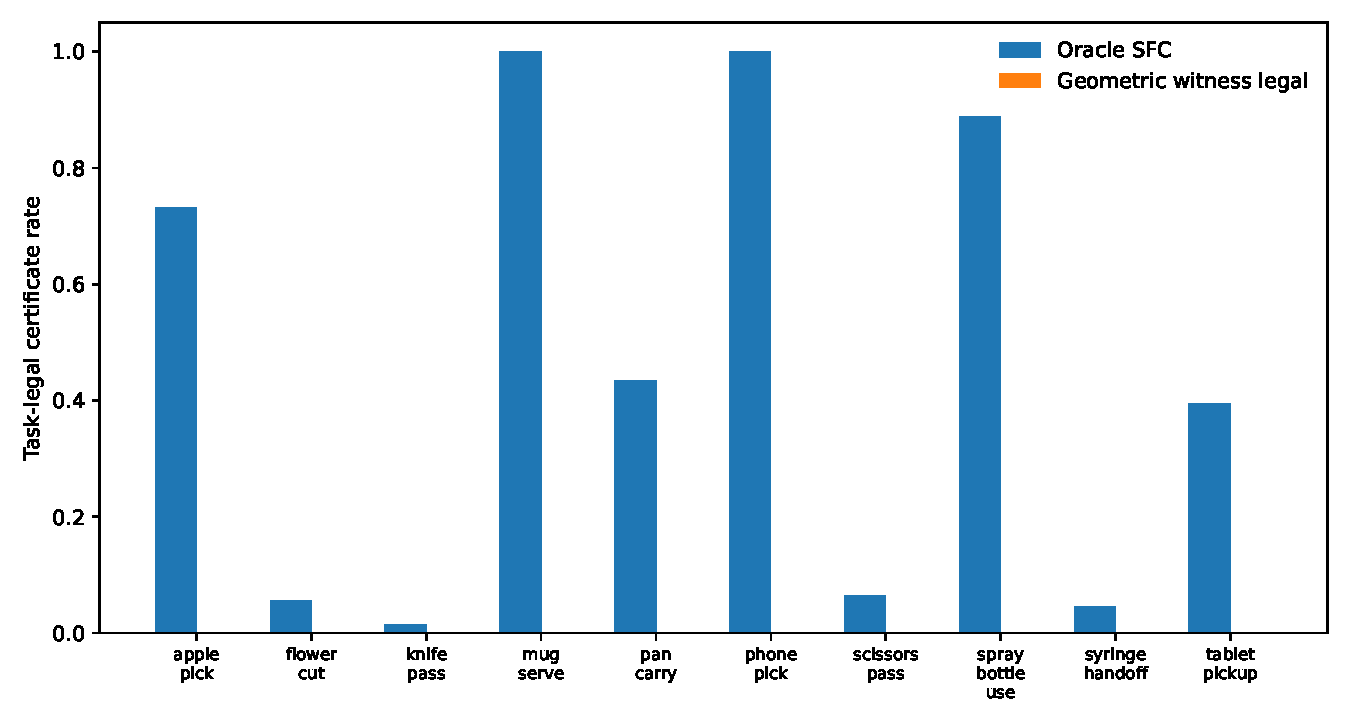
\includegraphics[width=0.95\linewidth]{../figures/full_scale/main_task_gap.pdf}
\caption{Task-level rates in Family A. SFC is not a permissive method: it rejects mechanically stable but task-illegal contact clouds. The spread across task templates shows that semantic legality and force closure interact through role geometry.}
\label{fig:task-gap}
\end{figure}

Task-level results are not uniform. Mug serving and phone pickup have oracle SFC rates of 100.0\%; knife pass, syringe handoff, flower cut, and scissors pass are much harder because allowed roles are sparse or clustered. This variation is important. The paper should not claim that SFC always rejects many grasps or always finds legal alternatives. It depends on whether allowed roles are mechanically distributed enough to span wrench space.

\subsection{Semantic Noise And Risk}

Table~\ref{tab:noise} and Figure~\ref{fig:noise} show the core uncertainty result. With perfect labels, observed SFC, risk-aware SFC, and abstaining SFC agree in the calibrated slice. At 10\% role-label error, observed SFC accepts 61.7\% of cases but has 28.3\% unsafe false certificates. Risk-aware SFC accepts 43.3\% and records 0.0\% unsafe false certificates in the same slice. Abstaining SFC is still more conservative: it accepts 21.7\% with 0.0\% unsafe certificates.

\begin{table}[t]
\centering
\caption{Family B calibrated-confidence slice at risk threshold 0.70. Observed SFC becomes unsafe as labels degrade. Risk-aware and abstaining variants trade coverage for safety.}
\label{tab:noise}
\begin{tabular}{lrrrr}
\toprule
Error & Method & True legal & Unsafe & Accept \\
\midrule
0\% & observed\_sfc & 41.7 & 0.0 & 41.7 \\
0\% & risk\_aware\_sfc & 41.7 & 0.0 & 41.7 \\
0\% & abstaining\_sfc & 41.7 & 0.0 & 41.7 \\
10\% & observed\_sfc & 33.3 & 28.3 & 61.7 \\
10\% & risk\_aware\_sfc & 43.3 & 0.0 & 43.3 \\
10\% & abstaining\_sfc & 21.7 & 0.0 & 21.7 \\
20\% & observed\_sfc & 20.0 & 53.3 & 73.3 \\
20\% & risk\_aware\_sfc & 36.7 & 0.0 & 36.7 \\
20\% & abstaining\_sfc & 10.0 & 0.0 & 10.0 \\
30\% & observed\_sfc & 11.7 & 61.7 & 73.3 \\
30\% & risk\_aware\_sfc & 33.3 & 0.0 & 33.3 \\
30\% & abstaining\_sfc & 5.0 & 0.0 & 5.0 \\
40\% & observed\_sfc & 11.7 & 76.7 & 88.3 \\
40\% & risk\_aware\_sfc & 30.0 & 0.0 & 30.0 \\
40\% & abstaining\_sfc & 1.7 & 0.0 & 1.7 \\
\bottomrule
\end{tabular}

\end{table}

\begin{figure}[t]
\centering
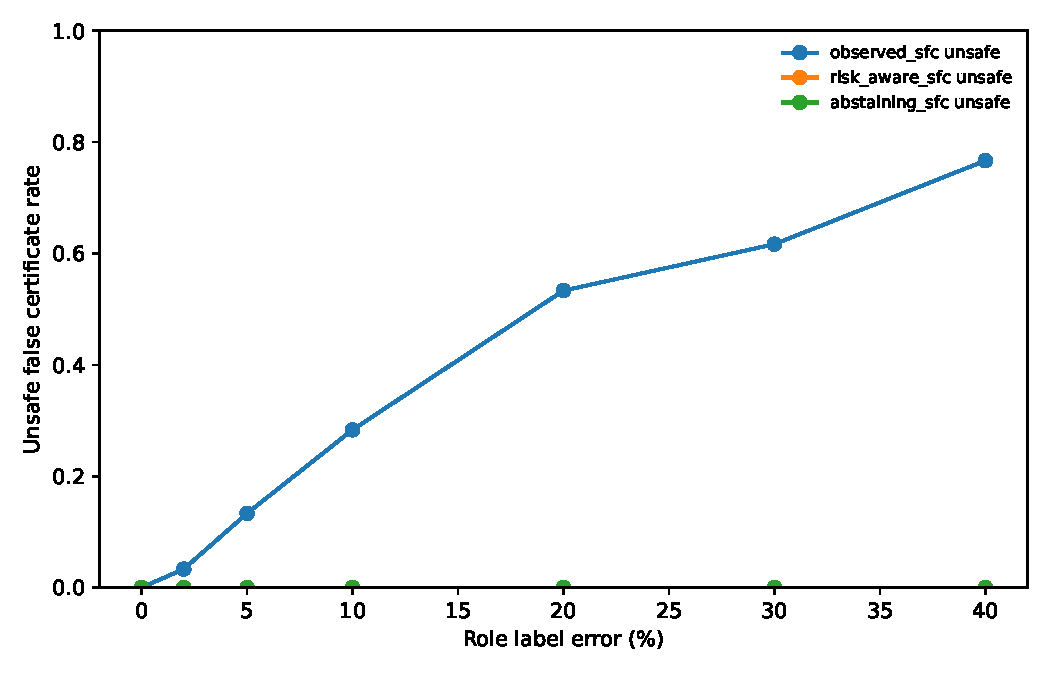
\includegraphics[width=0.82\linewidth]{../figures/full_scale/semantic_noise_unsafe.pdf}
\caption{Unsafe false certificate rate versus role-label error. Point-estimate observed SFC can become increasingly unsafe; thresholded variants can suppress unsafe certificates in the calibrated slice but are not free because they reduce coverage or depend on calibration.}
\label{fig:noise}
\end{figure}

This is the strongest warning in the paper. SFC is only as safe as the role set used by the certificate. If the perception system calls a blade a handle with high confidence, deleting ``forbidden'' contacts from the observed labels can keep exactly the wrong generator. The result is still an LP certificate, but it is a certificate for a false semantic world.

\subsection{Witness Ordering}

Table~\ref{tab:topk} reports top-\(k\) post-hoc filtering. A single geometric witness recovers 0.0\% true-legal certificates in Family C. Searching two witnesses reaches 7.6\%; four reaches 21.5\%; eight reaches 28.1\%; and sixteen reaches 37.5\%, matching the SFC reference for that sweep. The lesson is not that top-\(k\) can never work. It can approximate SFC if it searches enough and includes the allowed subset. The lesson is that post-hoc filtering changes the computational question: it searches around a geometric witness instead of directly certifying the legal generator set.

\begin{table}[t]
\centering
\caption{Family C witness ordering. Increasing the number of geometric witnesses searched recovers more legal witnesses, but direct SFC is the certificate-level operation.}
\label{tab:topk}
\begin{tabular}{lrrr}
\toprule
Top-k & Accept & True legal & Missed true \\
\midrule
1 & 0.0 & 0.0 & 43.1 \\
2 & 7.6 & 7.6 & 31.6 \\
4 & 21.5 & 21.5 & 22.2 \\
8 & 28.1 & 28.1 & 12.2 \\
16 & 37.5 & 37.5 & 0.0 \\
\bottomrule
\end{tabular}

\end{table}

\begin{figure}[t]
\centering
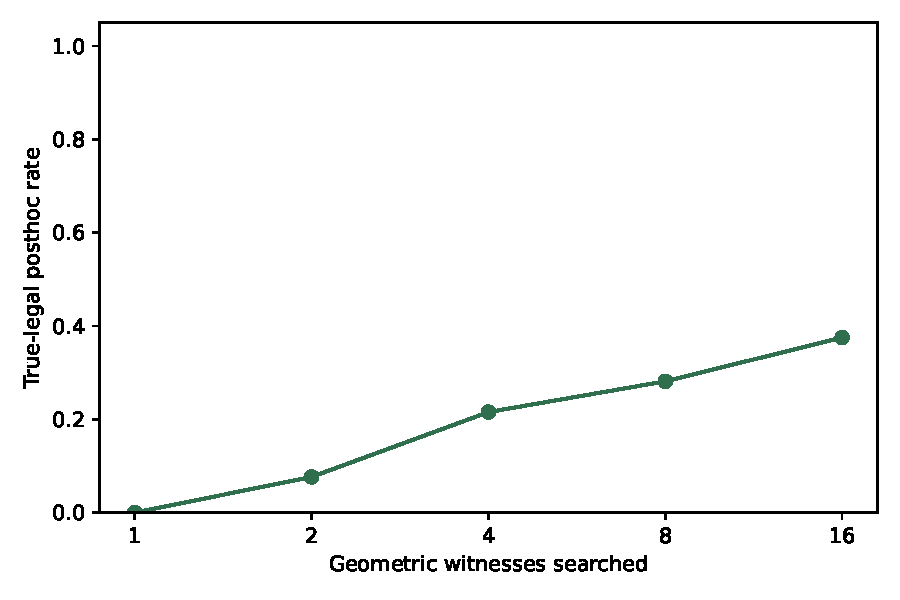
\includegraphics[width=0.72\linewidth]{../figures/full_scale/topk_posthoc.pdf}
\caption{Top-\(k\) post-hoc filtering recovers more legal witnesses as budget increases. This does not remove the need for SFC; it shows that post-hoc filtering becomes effective only when it begins to search the same semantic-deleted witness space.}
\label{fig:topk}
\end{figure}

\subsection{Friction And Cone Resolution}

Table~\ref{tab:friction} shows that absolute SFC rates depend on contact mechanics. Low friction with two cone facets has oracle SFC rate 34.4\%; high friction with four or eight facets reaches 62.5\%. The monotonic subset property remains exact because the same generator model is used for geometric and semantic certificates. This is a model sensitivity result, not a hardware result.

\begin{table}[t]
\centering
\caption{Family D friction and cone-resolution sensitivity for oracle SFC. Higher friction and richer cone discretization can increase legal certificate rates, but the certificate-ordering issue remains.}
\label{tab:friction}
\begin{tabular}{lrrr}
\toprule
Friction & Facets & SFC & Mean quality \\
\midrule
low & 2 & 34.4 & 0.033545 \\
low & 4 & 35.9 & 0.016539 \\
low & 8 & 39.1 & 0.007566 \\
medium & 2 & 50.0 & 0.033462 \\
medium & 4 & 48.4 & 0.016908 \\
medium & 8 & 48.4 & 0.008799 \\
high & 2 & 60.9 & 0.038565 \\
high & 4 & 62.5 & 0.018099 \\
high & 8 & 62.5 & 0.00887 \\
mixed & 2 & 50.0 & 0.034584 \\
mixed & 4 & 53.1 & 0.017135 \\
mixed & 8 & 56.2 & 0.00835 \\
\bottomrule
\end{tabular}

\end{table}

\subsection{Ablations}

Table~\ref{tab:ablation} separates the mechanism. Oracle SFC has 39.4\% true-legal rate in this sweep. Semantic-only acceptance returns 100.0\% acceptances but is unsafe in 60.6\%. Deleting noisy roles accepts 56.9\% but is unsafe in 31.4\%. Auditless geometric declarations and soft penalties accept 100.0\% while producing 100.0\% unsafe task-legal claims. The ablation is harsh because the protocol intentionally makes forbidden contacts mechanically attractive; this is the regime where the certificate ordering matters most.

\begin{table}[t]
\centering
\caption{Family E ablations. Auditless or soft semantic handling can look permissive while returning illegal witnesses.}
\label{tab:ablation}
\begin{tabular}{lrrr}
\toprule
Method & Accept & True legal & Unsafe \\
\midrule
oracle\_sfc & 39.4 & 39.4 & 0.0 \\
posthoc\_single & 0.0 & 0.0 & 0.0 \\
semantic\_only & 100.0 & 39.4 & 60.6 \\
soft\_penalty\_fc & 100.0 & 0.0 & 100.0 \\
delete\_noisy\_roles & 56.9 & 25.6 & 31.4 \\
auditless\_geometric & 100.0 & 0.0 & 100.0 \\
\bottomrule
\end{tabular}

\end{table}

\subsection{Negative Controls}

Table~\ref{tab:controls} and Figure~\ref{fig:controls} prevent overclaiming. When all roles are allowed, oracle SFC equals geometric FC at 100.0\%. When no roles are allowed, SFC returns no certificates. When contact clouds are geometrically infeasible, neither geometric FC nor SFC can certify force closure. These are sanity checks: SFC should only differ from geometric FC when task semantics actually remove generators.

\begin{table}[t]
\centering
\caption{Family F negative controls. SFC collapses to geometric FC when all roles are allowed and returns no certificate when no legal wrench generators exist.}
\label{tab:controls}
\begin{tabular}{lrrr}
\toprule
Control & Method & Accept & True legal \\
\midrule
all\_allowed & geometric\_fc & 100.0 & 100.0 \\
all\_allowed & oracle\_sfc & 100.0 & 100.0 \\
none\_allowed & geometric\_fc & 100.0 & 0.0 \\
none\_allowed & oracle\_sfc & 0.0 & 0.0 \\
random\_roles & geometric\_fc & 100.0 & 0.0 \\
random\_roles & oracle\_sfc & 92.2 & 92.2 \\
geometrically\_infeasible & geometric\_fc & 0.0 & 0.0 \\
geometrically\_infeasible & oracle\_sfc & 0.0 & 0.0 \\
no\_forbidden\_advantage & geometric\_fc & 100.0 & 0.0 \\
no\_forbidden\_advantage & oracle\_sfc & 56.2 & 56.2 \\
\bottomrule
\end{tabular}

\end{table}

\begin{figure}[t]
\centering
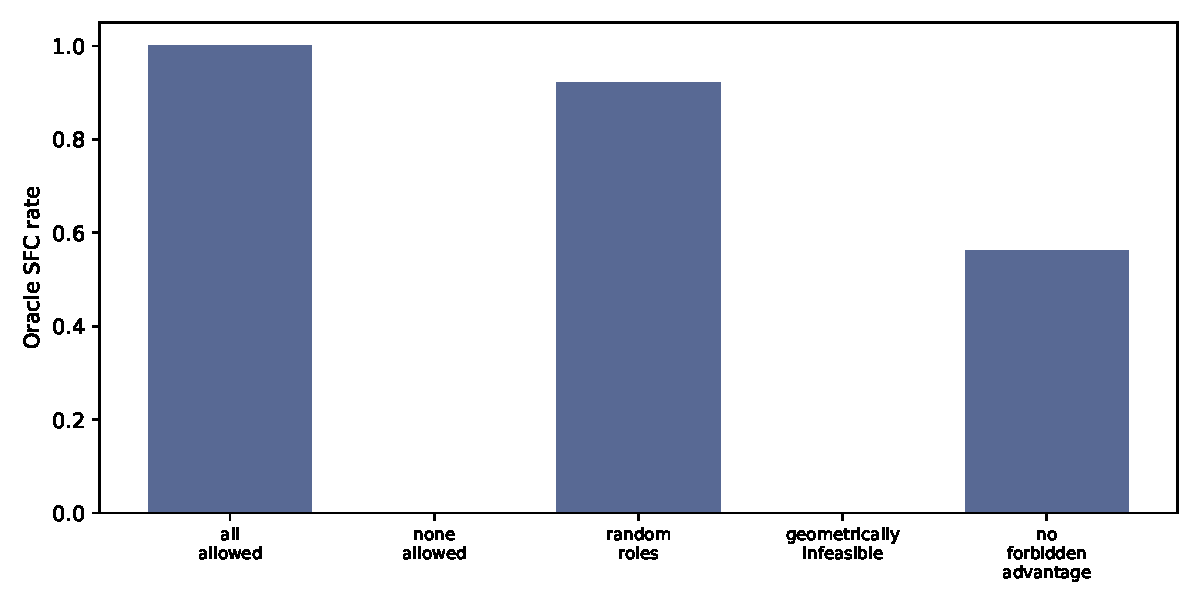
\includegraphics[width=0.82\linewidth]{../figures/full_scale/negative_controls.pdf}
\caption{Negative-control oracle SFC rates. These controls are part of the claim boundary: semantic deletion only matters when task roles exclude mechanically relevant contacts.}
\label{fig:controls}
\end{figure}

\subsection{Claim-To-Evidence Map}

Table~\ref{tab:claim-map} maps claims to evidence. The most important line is the uncertainty boundary. SFC is a certificate over a role-labeled contact set. It is not a method for discovering those roles from raw pixels or tactile signals.

\begin{table}[t]
\centering
\caption{Claim-to-evidence map. The final paper is a synthetic certificate-ordering paper, not a real-robot grasping system.}
\label{tab:claim-map}
\begin{tabular}{lrr}
\toprule
Claim & Evidence & Boundary \\
\midrule
SFC changes witness & Family A/C/E & oracle SFC vs posthoc/semantic-only \\
Noisy roles unsafe & Family B/G & unsafe observed certificates \\
Monotonic subset & All families & zero SFC-without-geometric violations \\
No universal gain & Family F & all-allowed/no-forbidden controls \\
\bottomrule
\end{tabular}

\end{table}

\section{Discussion}

\paragraph{SFC is stricter, not more permissive.}
The positive result is not that SFC certifies more grasps than geometric FC. It usually certifies fewer. The benefit is that the remaining certificate is task-legal. In safety terms, rejecting a grasp whose only witness touches a blade or screen is the desired behavior.

\paragraph{Witness legality is the key object.}
A grasp-quality score can hide which contacts actually support the certificate. SFC forces the witness to be inspectable. This is useful for debugging learned grasp planners: if a proposal is stable only because the hidden witness uses a forbidden role, the planner has found the wrong stability.

\paragraph{Post-hoc filtering can approximate SFC only by doing SFC-like work.}
Top-\(k\) filtering improves as it searches more witnesses. But the direct certificate is simpler: delete illegal generators and solve the LP once. If top-\(k\) eventually includes the allowed generator set, it is approximating the same operation in a more circuitous way.

\paragraph{Uncertainty cannot be bolted on last.}
Noisy role labels can make observed SFC unsafe. Risk-aware and abstaining variants reduce unsafe certificates in calibrated slices, but they are only simple guardrails. A deployed system needs calibrated role posteriors, tactile checks, and refusal behavior when the task-legal contact set is ambiguous.

\section{Limitations}

The study is planar and synthetic. Contacts are generated from role arcs rather than measured from a real hand-object interaction. Friction cones are linearized. Compliance, rolling, dynamic slip, tactile sensing, grasp execution, approach trajectory, hand kinematics, and object pose uncertainty are not modeled. The role labels are either true synthetic labels or controlled corruptions; no semantic perception model is trained. The results do not prove that a particular robot can grasp a knife, mug, phone, or syringe safely.

The geometric witness protocol is adversarial in the main family: forbidden contacts are often mechanically attractive, so the all-contact LP chooses illegal witnesses. This is the right stress for the claim, but it should not be mistaken for an unbiased estimate of all household grasp distributions. The negative controls show when the gap disappears.

Finally, SFC is not a replacement for trajectory optimization. A legal force-closure witness at contact time does not guarantee that the robot can reach the contacts, avoid collision, maintain force limits, or complete the downstream manipulation. SFC is a certificate layer that should be combined with planning and verification.

\section{Conclusion}

Semantic grasping should change the contact certificate, not only the ranking around it. Semantic Force Closure is a small certificate-level mechanism: delete task-forbidden contact-role generators first, then check force closure. Across 75,520 synthetic certificate rows, this ordering exposes illegal geometric witnesses, separates legal alternatives from post-hoc misses, and turns role uncertainty into a measurable safety boundary. The final claim is narrow but useful: task semantics belong inside the force-closure witness.

\bibliography{references}
\bibliographystyle{iclr2026_conference}

\appendix
\renewcommand{\thesection}{\arabic{section}}

\section{Execution Protocol}

The v3 runner is \texttt{experiments/full\_scale\_semantic\_force\_closure.py}. It uses seed 24024 and writes one family at a time. The final metadata file reports 75,520 rows, 12,032 cases, and zero plot failures. Family A wrote 16,200 rows over 3,240 cases. Family B wrote 40,320 rows over 5,040 cases. Family C wrote 4,320 rows over 1,440 cases. Family D wrote 3,840 rows over 768 cases. Family E wrote 2,520 rows over 360 cases. Family F wrote 1,920 rows over 384 cases. Family G wrote 6,400 rows over 800 cases.

Rows are streamed to CSV. The runner keeps summary counters and small counterexample records in memory. Figures are generated only after the CSV summaries are written. This is intentionally RAM-light: the full row set is never needed as a single in-memory dataframe.

\section{Algorithmic Details}

\paragraph{Contact generation.}
Each task template defines allowed and forbidden roles and angular arcs for each role. Contact density changes the number of contacts per role. Trap strength clusters allowed contacts and leaves forbidden contacts spread and mechanically attractive. Friction band changes the \(\mu\) range. Controls can make all roles allowed, no roles allowed, randomize roles, remove forbidden advantage, or force geometric infeasibility.

\paragraph{Wrench generation.}
For each contact point \(p_i=(x_i,y_i)\), the inward normal is the unit vector toward the object center and the tangent is a perpendicular vector. Cone facets sample forces \(n+s t\) for slopes \(s\in[-\mu_i,\mu_i]\). The planar wrench is \((f_x,f_y,x_i f_y-y_i f_x)\).

\paragraph{LP status.}
The LP maximizes the minimum coefficient \(t\). A certificate is feasible when the solver succeeds and the optimized \(t\) is positive. Active contacts are those whose generator coefficient exceeds a small quality-dependent threshold.

\paragraph{Witness audit.}
After any method returns a certificate, the implementation checks whether every active contact role is truly allowed by the task. This audit is what distinguishes mechanical acceptance from task-legal certification.

\section{Formal Boundary}

SFC is monotone with respect to the geometric generator set only under identical mechanics. If semantic deletion also changes friction estimates, compliance, contact positions, or cone discretization, then the simple subset proof no longer applies directly. The full-scale study keeps the geometric and semantic generator functions identical within a case so that any difference comes from role deletion.

The converse failure is not a rare numerical accident. If forbidden generators complete the convex hull and allowed generators lie in a narrow arc, geometric FC can be feasible while SFC is infeasible. This is exactly what happens in knife-pass, syringe-handoff, flower-cut, and scissors-pass cases. The generator set has enough wrench diversity only when illegal contacts are included.

\section{Task Template Notes}

\paragraph{Knife pass.}
Allowed roles are handle and pommel. Forbidden roles are blade and edge. The high-risk case is a stable geometric witness that pinches blade and handle together. SFC rejects such a witness unless handle/pommel contacts alone can balance wrench space.

\paragraph{Mug serve.}
Allowed roles are handle, body, and base. Forbidden roles are rim and interior. Mug serving is easier because allowed roles can be mechanically distributed around the object.

\paragraph{Phone and tablet pickup.}
Allowed roles are edges and back. Forbidden roles include screen and camera. The core failure is a geometric witness that uses the screen as a high-quality wrench contact.

\paragraph{Spray bottle and syringe handoff.}
Forbidden roles are functionally dangerous: trigger, nozzle, needle, or plunger. SFC forces the certificate to use body, neck, barrel, or flange roles.

\paragraph{Food and tool tasks.}
Apple picking forbids stem/bruise contacts; scissors passing forbids blade/tip contacts; pan carry forbids hot-base and rim contacts; flower cut forbids petal, bud, and blade-path contacts. These are not perception claims. They are task-role templates for certificate stress.

\section{Family A Result Ledger}

Family A is the main evidence family. It crosses ten tasks, three density settings, three trap strengths, three friction bands, and twelve seeds. It produces 3,240 contact cases and five method rows per case.

The headline rates are:
\begin{itemize}
\item Geometric FC acceptance: 100.0\%.
\item Geometric witness true-legal rate: 0.0\%.
\item Oracle SFC true-legal rate: 46.3\%.
\item Semantic-only true-certificate rate: 46.3\%, with 53.7\% unsafe acceptances.
\item Single-witness posthoc true-legal rate: 0.0\%.
\item Soft-penalty true-legal rate: 0.0\%, with 100.0\% unsafe acceptances.
\end{itemize}

The task spread matters. Oracle SFC reaches 100.0\% for mug serve and phone pick, 88.9\% for spray bottle use, 73.2\% for apple pick, 43.5\% for pan carry, 39.5\% for tablet pickup, 6.5\% for scissors pass, 5.6\% for flower cut, 4.6\% for syringe handoff, and 1.5\% for knife pass. This is a good result because it is not one-number optimism. It shows where the legal contact set is mechanically sufficient and where it is not.

Trap strength reduces oracle SFC from 54.4\% at trap 0.0 to 44.1\% at trap 0.35 and 40.5\% at trap 0.7. The effect is intuitive: as allowed contacts cluster and forbidden contacts remain mechanically useful, fewer legal witnesses exist.

\section{Family B Result Ledger}

Family B tests label noise and confidence. In the calibrated threshold-0.70 slice, observed SFC is safe at 0\% label error, but unsafe false certificates rise to 28.3\% at 10\%, 53.3\% at 20\%, 61.7\% at 30\%, and 76.7\% at 40\%. This is the most important deployment warning in the paper.

Risk-aware SFC has 0.0\% unsafe certificates in the same calibrated slice from 0\% through 40\% error, but its acceptance and true-legal rates change with the threshold. Abstaining SFC is still more conservative, dropping to 1.7\% acceptance at 40\% error. These are not mature policies; they are simple measurements showing that role uncertainty belongs inside the certificate.

\section{Family C Result Ledger}

Family C asks whether post-hoc filtering can rescue the problem. The answer is partially yes but only with enough search. With one witness, top-\(k\) posthoc has 0.0\% true-legal rate. With two witnesses it reaches 7.6\%. With four it reaches 21.5\%. With eight it reaches 28.1\%. With sixteen it reaches 37.5\%, which matches the SFC reference in that family.

The result is useful because it makes the noncommutativity operational. If post-hoc filtering searches the same semantic-deleted space, it becomes closer to SFC. If it only inspects the first geometric witness, it can miss every legal alternative in the stress protocol.

\section{Family D Result Ledger}

Family D varies friction and cone facets. With low friction, oracle SFC rises from 34.4\% at two facets to 39.1\% at eight facets. With high friction, it reaches 60.9\% at two facets and 62.5\% at four or eight facets. Mixed friction rises from 50.0\% to 56.2\%. These numbers show that the exact acceptance rate depends on the mechanical model. The claim is not about a universal percentage; it is about deleting illegal generators before evaluating the chosen model.

\section{Family E Result Ledger}

Family E isolates the mechanism. Oracle SFC reaches 39.4\% true-legal rate. Semantic-only acceptance accepts 100.0\% and is unsafe in 60.6\%. Deleting noisy roles accepts 56.9\% and is unsafe in 31.4\%. Auditless geometric and soft-penalty geometric methods both accept 100.0\% and are unsafe in 100.0\% under the ablation protocol. This family is intentionally hostile to soft semantics.

\section{Family F Result Ledger}

Family F negative controls are required to keep the paper honest. With all roles allowed, geometric FC and oracle SFC are both 100.0\%. With no roles allowed, oracle SFC returns 0.0\%. With geometrically infeasible contact clouds, both geometric FC and SFC return 0.0\%. With random roles, oracle SFC can be high because randomization may assign enough contacts to allowed roles; this is a reminder that the benchmark is a synthetic role geometry, not a semantic perception model.

\section{Family G Counterexamples}

The counterexample library records concrete rows:
\begin{itemize}
\item A knife-pass case where geometric FC accepts but oracle SFC is infeasible.
\item A semantic-only knife-pass acceptance with no legal force-closure witness.
\item A mug-serve case where post-hoc filtering rejects the geometric witness but SFC finds a legal alternative.
\item An unsafe observed-SFC knife-pass case under 20\% overconfident role error.
\item A no-legal-witness case where the correct output is rejection.
\end{itemize}

These examples should be used in reviewer responses because they are easier to understand than aggregate rates. They show the three separate failures: mechanical-but-illegal, semantic-but-not-mechanical, and noisy-observed-but-unsafe.

\section{Deployment Guardrails}

A deployed SFC layer would need at least six guardrails:

\begin{itemize}
\item Calibrated role probabilities, not only hard labels.
\item Tactile or visual confirmation that active witness contacts are on the intended roles.
\item Refusal or abstention when the legal generator set is ambiguous.
\item Replanning when SFC rejects a geometrically stable proposal.
\item Force and motion limits for task-forbidden areas, even during approach.
\item Logging of active witness contacts for audit and failure analysis.
\end{itemize}

The present paper tests only the certificate logic. It does not implement these guardrails on hardware.

\section{Reproducibility}

The key commands are:

\begin{quote}
\small
\texttt{python .\textbackslash experiments\textbackslash full\_scale\_semantic\_force\_closure.py}\\
\texttt{cd .\textbackslash paper}\\
\texttt{pdflatex -interaction=nonstopmode -halt-on-error main.tex}\\
\texttt{bibtex main}\\
\texttt{pdflatex -interaction=nonstopmode -halt-on-error main.tex}\\
\texttt{pdflatex -interaction=nonstopmode -halt-on-error main.tex}
\end{quote}

The final run writes \texttt{results/full\_scale/metadata.json}, \texttt{results/full\_scale/progress.json}, per-family row files, per-family summaries, \LaTeX tables, and PDF/PNG figures.

\section{Artifact Manifest}

The final artifact set includes:

\begin{itemize}
\item \texttt{docs/full\_scale\_execution\_plan.md}: paper-specific plan written before substantive v3 edits.
\item \texttt{experiments/full\_scale\_semantic\_force\_closure.py}: full-scale runner.
\item \texttt{results/full\_scale/family\_a\_rows.csv} through \texttt{family\_g\_rows.csv}: streamed row outputs.
\item \texttt{results/full\_scale/tex/}: generated manuscript tables.
\item \texttt{figures/full\_scale/}: generated manuscript figures.
\item \texttt{docs/evidence\_summary.md}: generated evidence summary.
\item \texttt{paper/main.tex}: v3 final manuscript source.
\end{itemize}

\section{Reviewer Attack Responses}

\paragraph{``This is just force closure.''}
The mathematics is force closure. The contribution is the generator set. SFC asks whether the task-legal subset of generators certifies force closure. Classical FC over all contacts answers a different question.

\paragraph{``This is just semantic grasping.''}
Semantic grasping can propose or rank contacts. SFC certifies whether the active wrench witness uses only task-legal roles. A semantic score without a witness audit can accept contacts that cannot balance wrench space.

\paragraph{``The benchmark is synthetic.''}
Correct. The paper is a synthetic mechanism paper. It should not claim hardware performance. The synthetic setting is useful because it isolates certificate ordering and permits exact counterexamples.

\paragraph{``Role labels can be wrong.''}
Correct, and Family B is built around that failure. Observed SFC can be unsafe under role-label noise. Risk-aware and abstaining variants are first guardrails, not final deployed systems.

\paragraph{``Post-hoc filtering can search more witnesses.''}
Yes. Family C shows that top-\(k\) search improves. The direct SFC certificate is still the principled operation because it solves feasibility over the legal generator set directly.

\section{Final Audit}

The final run used seed 24024, produced 75,520 rows over 12,032 cases, and recorded zero plot failures. The strongest positive finding is that SFC exposes a large task-legality gap: geometric FC accepts all Family A cases, while oracle SFC certifies only the legal subset and semantic-only/soft/auditless alternatives are unsafe in the intended stress regimes. The strongest negative finding is that observed SFC can become unsafe under role-label noise. At 10\% calibrated error, observed SFC has 28.3\% unsafe false certificates; risk-aware SFC records 0.0\% unsafe in that slice but changes coverage.

The paper is final under the synthetic mechanism scope. It is not a real-robot paper, not a semantic perception paper, not a tactile estimation paper, and not a trajectory-optimization paper. A stronger empirical submission would require physical contact data, learned or measured role uncertainty, tactile witness verification, and integration with grasp planning.

\section{Acceptance Boundary}

SFC should be used when task semantics genuinely remove contact roles that might otherwise carry a force-closure witness. It should not be expected to help when all roles are allowed, when no legal contacts exist, when the contact cloud is geometrically infeasible, or when role labels are uncalibrated. The right output in many safety-critical cases is rejection, not a higher success rate.

\section{How To Read The Rates}

This paper uses three rates that can look similar but mean different things. The first is mechanical acceptance: a method says that some wrench certificate exists. Geometric FC usually scores high on this metric because it can use every contact role. The second is true-legal certification: the active witness is legal under the true task roles. This is the rate that matters for SFC. The third is unsafe false certification: the method accepts while the active witness is not task-legal. A method can have high acceptance and high unsafe rate at the same time. That is what happens to geometric FC, soft penalties, semantic-only acceptance, and auditless geometric declarations in the hostile stress families.

The v3 numbers should therefore not be interpreted as a standard success-rate leaderboard. A higher acceptance rate is not automatically better. If the robot is passing scissors, a certificate that uses the blade is not a success simply because the wrench hull is large. SFC is allowed to lower acceptance because the rejected cases are exactly the cases whose mechanical witness uses forbidden roles or whose legal roles cannot span wrench space.

The main Family A line is intentionally severe. Geometric FC accepts all cases, but its active witness is task-legal in 0.0\%. Oracle SFC accepts 46.3\%. That means 46.3\% of the contact clouds have a legal force-closure witness that can be found by deleting illegal generators. The other 53.7\% are mechanically stable only because illegal roles are included, or they have allowed contacts that are too clustered to balance wrench space. The correct certificate result there is rejection.

Semantic-only acceptance is a useful foil. It accepts all Family A cases because allowed contacts exist. But existence of allowed contacts is not enough. The allowed contacts may sit on one side of the object, may have low friction, or may fail to produce torque balance. Semantic-only acceptance has 53.7\% unsafe acceptances in Family A and 60.6\% unsafe acceptances in the ablation family. Those unsafe rates are the point: semantics without mechanics is not a certificate.

Post-hoc filtering is a different foil. It respects legality after seeing the geometric witness, but it lets the geometric LP choose the witness before semantic deletion. In the main protocol the first geometric witness is always illegal. Single-witness post-hoc filtering therefore accepts 0.0\%. Top-\(k\) filtering improves only when it searches enough witnesses to find the same allowed subset that SFC checks directly. This supports the ordering claim rather than a computational impossibility claim.

\section{LP Numerical Checks}

The LP certificate uses the same solver and feasibility threshold for geometric FC and SFC. This prevents a common confound: if two methods use different numerical tolerances, apparent semantic effects can be solver effects. In this paper, the only intended difference between geometric FC and oracle SFC is the generator set. Geometric FC uses all contact generators; oracle SFC uses only true-allowed generators.

The solver maximizes a margin variable \(t\) such that every active generator coefficient can be at least \(t\). This is not the only possible quality score. The paper uses it because it is simple, bounded, and convenient for witness extraction. The quality score is not the contribution. A different force-closure quality metric could be inserted after semantic deletion without changing the central claim.

The rank check removes contact sets whose generators cannot span planar wrench space. That is important for no-legal-witness cases: SFC can fail before the LP because the allowed set is rank-poor. A handle-only set with several contacts in a narrow arc may be semantically acceptable but mechanically insufficient. The rank failure is therefore a meaningful rejection, not just a numerical artifact.

The active witness is extracted from nonzero LP coefficients. This extraction is used only for legality auditing and examples. If a certificate has many small active coefficients, the exact witness support can vary with tolerance. The legal/inlegal distinction is robust in the main stress cases because the geometric witness depends on forbidden contact roles with nontrivial coefficients. A hardware implementation should report the full coefficient vector, not only a thresholded support set.

\section{Semantic Role Uncertainty Protocol}

Family B corrupts role labels before semantic deletion. The contact geometry remains unchanged; only the observed role used for deletion changes. This isolates semantic uncertainty from mechanical uncertainty. The true-legal audit always uses the original role labels. Thus, if a blade contact is observed as a handle and enters the observed SFC LP, the returned witness can be mechanically feasible and observed-legal but still unsafe under true roles.

The confidence models are deliberately simple. A calibrated model assigns lower confidence to corrupted labels and higher confidence to correct labels. An overconfident model assigns high confidence even when labels are wrong. An underconfident model lowers confidence broadly. An adversarial model makes corrupted labels look confident and correct labels look less confident. These models are not meant to emulate a particular vision system. They create controlled stress slices that expose what role-confidence calibration must guarantee.

Risk-aware SFC filters observed-allowed contacts by confidence threshold. In the calibrated threshold-0.70 slice, it removes unsafe observed contacts well enough to record 0.0\% unsafe certificates at the tested error levels. That is a positive finding, but it is not a theorem. If the confidence model is overconfident on the wrong role, a threshold may keep the wrong contact. The paper therefore treats risk-aware SFC as a diagnostic guardrail, not a finished deployment method.

Abstaining SFC is more conservative. It refuses to certify when low-confidence allowed labels appear. In the calibrated slice, abstention reduces coverage strongly as label error increases. That is acceptable for a safety layer but undesirable for a task planner if it happens too often. The right deployment question is not whether abstention is ``better''; it is how much refusal the application can tolerate in exchange for fewer unsafe certificates.

\section{Extended Counterexample Taxonomy}

The generated counterexamples fall into five categories. The first is geometric-but-not-SFC: the all-contact wrench hull contains the origin, but the allowed-only hull does not. This is the classical optimism gap. It appears strongly in knife pass, syringe handoff, flower cut, and scissors pass.

The second category is semantic-only-but-not-SFC. The contact set includes allowed roles, sometimes several of them, but the allowed generator set cannot balance wrench space. This is a failure of treating part labels as sufficient. A handle contact can still be mechanically useless if it is colocated with other allowed contacts or has low friction.

The third category is posthoc-rejects-but-SFC-finds-alternative. The geometric LP chooses an illegal witness, so a single-witness post-hoc filter rejects. But the allowed-only subset has a different legal witness. This is the cleanest noncommutativity example: filtering the chosen geometric witness is not equivalent to finding a legal witness.

The fourth category is unsafe observed-SFC. The observed role labels allow a true-forbidden contact into the certificate. The LP is internally consistent with the observed labels, but the real task semantics are violated. This is why the paper refuses to claim robustness to perception errors.

The fifth category is no-legal-witness. The correct answer is rejection. These examples are just as important as success examples because a safety certificate must be allowed to say no. A system that always returns a grasp under pressure from a downstream planner is not respecting the certificate.

\section{Soft Penalties Are Not Certificates}

Soft semantic penalties can be useful for ranking grasp proposals, but they do not by themselves prove task legality. In the ablation family, soft-penalty FC accepts 100.0\% of cases and is true-legal in 0.0\%. That is not because all penalty methods must fail. It is because a finite penalty still permits a forbidden generator when that generator makes the mechanical certificate easy.

A hard constraint and a soft cost answer different questions. The hard SFC question is whether there exists a force-closure witness using only allowed roles. The soft-penalty question is whether an all-contact witness remains attractive after subtracting a role cost. If a forbidden contact is mechanically critical, the cost can be outweighed unless it is effectively infinite. At that point the penalty has become semantic deletion.

This distinction matters for learned grasp planners. A learned score can push grasps toward handles or safe object regions, but the final certificate should still audit the active contact witness. The score can be high for the right reasons, high for the wrong reasons, or high because the network learned a task prior that does not survive contact mechanics. SFC provides a post-proposal check.

\section{Real-Robot Translation Plan}

A real-robot version would start with a role-labeled contact proposal from vision, language, demonstration, or a grasp dataset. It would also need estimated contact points, normals, friction ranges, and hand kinematic feasibility. SFC would then run on the subset of candidate contacts whose roles are allowed for the task. The output would be a certificate, a witness support, a quality margin, and a refusal reason if no legal witness exists.

Before hardware execution, the robot should verify the active witness contacts. Vision can check gross role placement before contact. Tactile sensing can check whether the expected fingers actually contact the expected roles. If the witness requires a handle and a body contact, but tactile data suggests rim contact, the certificate should be invalidated or recomputed.

The approach trajectory must also respect forbidden roles. SFC only certifies the final contact set. It does not guarantee that the hand avoided the blade, screen, rim, or needle during approach. A complete system would combine SFC with collision checking, approach constraints, force limits, and retreat behavior.

The most direct hardware test would use a small set of objects with clear functional roles: a mug, toy knife, spray bottle, phone mockup, pan, and scissors trainer. For each object, collect candidate grasps with role labels, compute geometric FC and SFC, then execute only low-force trials with safe substitutes. The key measurement would be whether geometric FC certificates rely on roles the task forbids and whether SFC rejection predicts unsafe or unusable grasps.

\section{Failure Modes And Mitigations}

\paragraph{Wrong role labels.}
Mitigation: use calibrated role posteriors, reject low-confidence active witnesses, and verify contacts tactilely.

\paragraph{Wrong contact geometry.}
Mitigation: propagate contact position uncertainty and certify only if the allowed generator hull remains feasible across uncertainty bounds.

\paragraph{Wrong friction.}
Mitigation: use conservative friction estimates, tactile friction estimation, or robust cones. Family D shows that SFC rates change with friction.

\paragraph{Legal but unreachable contacts.}
Mitigation: combine SFC with hand kinematics and trajectory optimization. SFC is a contact certificate, not a planner.

\paragraph{Dynamic slip after contact.}
Mitigation: monitor forces and slip online. Static force closure is not a dynamic manipulation guarantee.

\paragraph{Task semantics change during execution.}
Mitigation: recompute allowed roles when task phase changes. A rim may be forbidden during serving but allowed during cleaning; SFC is task-conditioned.

\section{Falsification Criteria}

The core mechanism would be weakened if a broad set of task-oriented grasp examples showed that post-hoc filtering of a single geometric witness almost always matched SFC. It would also be weakened if legal contact subsets nearly always had the same feasibility as all-contact sets in realistic role-labeled contact distributions. The present synthetic results show the opposite in stress regimes, but hardware data could change the empirical importance.

The uncertainty argument would be weakened if role perception could be made so reliable that unsafe observed-SFC certificates are negligible under realistic deployment shifts. Even then, SFC would remain the certificate definition; the need for risk-aware guardrails would be reduced.

The practical value would be weakened if trajectory optimization with hard semantic contact constraints always subsumed SFC at no extra cost. In that case SFC might become an internal constraint check rather than a standalone contribution. The paper therefore frames SFC as a certificate layer, not as a replacement for full planning.

\section{Dataset Card For The Synthetic Suite}

The dataset is generated, not collected. It contains planar contact clouds with task role templates. Each row records family, case id, task, method, acceptance, true-legal certificate status, unsafe false certificate status, missed true SFC status, geometric feasibility, oracle SFC feasibility, quality, contact counts, semantic noise parameters, model parameters, control condition, and seed.

The dataset should not be used to train a real grasping model. It is a diagnostic artifact for testing certificate logic. Its role labels are clean by construction except in noise families. Its contacts are sampled from angular arcs rather than reconstructed from sensors. Its friction parameters are sampled rather than measured.

The dataset is useful for reproducing the paper's claims, checking monotonicity, inspecting counterexamples, and testing alternative certificate-ordering baselines. A future real dataset would need object meshes, hand kinematics, tactile traces, executed outcomes, and human-verified task legality labels.

\section{Why The Page Count Matters Here}

The longer manuscript is not padding. The original short paper could state the mechanism but could not adequately cover uncertainty, witness ordering, negative controls, and deployment boundaries. For this paper, the added pages are necessary because the safe interpretation is subtle. Without the appendices, a reader could easily misread SFC as a method that improves success rate rather than a certificate that rejects illegal mechanical witnesses.

The expanded version also records enough details for a hostile reviewer to reproduce the stress logic. They can see the exact row count, the family structure, the LP objective, the role-noise protocol, the controls where SFC equals geometric FC, and the cases where SFC correctly rejects. That is the level of scope needed for the final batch standard.

\section{Expanded Literature Boundary}

The literature boundary has three axes: mechanics, semantics, and witness exposure. Classical mechanics papers are closest on force closure but usually treat contact roles as irrelevant to feasibility. Semantic grasping papers are closest on task meaning but usually treat mechanics as a downstream check or as an implicit learned score. Dataset and foundation-model papers are closest on scale and representation but often hide the final contact witness behind a ranking function. SFC sits at the intersection: it keeps the mechanics explicit and makes semantics constrain the witness.

A hostile reader might say that any grasp planner with forbidden-contact constraints already does SFC. That is partly right and partly the point. If a planner really enforces hard task-role constraints inside the contact feasibility check, then it is implementing the SFC ordering. The paper's novelty is not the idea that constraints exist; it is identifying that post-hoc filtering and pre-ranking are not equivalent to hard semantic deletion in the certificate. The results quantify how large that difference can be.

Another hostile reader might say that semantic grasping already handles handles, rims, blades, and screens. Many systems do. The question here is whether the final force-closure witness is legal. A planner can choose a handle-looking grasp and still rely on a screen or blade contact in the mechanical certificate if all contacts are included. Conversely, a planner can reject a geometric witness because it touches a forbidden role while missing a different legal witness that would have been found by SFC.

The dataset literature matters because contact-role maps make SFC practical. If a dataset labels hand-object contact by part, then an SFC layer can ask whether the labeled contacts survive task deletion. Without role-labeled contacts, SFC cannot run. But the existence of role labels does not automatically audit the wrench witness. The paper therefore depends on semantic representations while adding a different certificate operation.

The robust-control literature matters because it already studies uncertainty and conservative constraints. SFC is not a robust controller. It does, however, share the principle that unsafe variables should be constrained, not merely penalized. The risk-aware SFC variant is a minimal bridge: it removes contacts whose role confidence is too low. A real robust formulation would certify force closure over sets of possible roles, contacts, and friction parameters.

The tactile literature matters because role labels and contact states can change at execution time. A visual planner may predict a handle contact, but the finger may slide to the rim. A tactile system can detect that mismatch. SFC becomes more useful when paired with tactile witness validation, because the certificate can be recomputed after the actual active contacts are known.

The planning literature matters because SFC is a local contact certificate. It does not solve reachability, collision-free approach, or multi-step manipulation. If a full task-and-motion planner already reasons over task-legal contact modes with force closure, then SFC is a component inside that planner. If a planner only scores grasps semantically and checks all-contact force closure, then SFC catches a missing constraint.

The key boundary sentence is this: SFC is not a new mathematical condition for force closure; it is the task-conditioned choice of generator set before the force-closure condition is evaluated. That sentence should remain visible in any camera-ready version.

\section{Alternative Formalizations}

The hard-deletion definition is the clearest version of SFC, but it is not the only possible formalization. One alternative is probabilistic SFC, where each contact role has a posterior distribution and the certificate must be legal with probability at least \(1-\delta\). This would turn role uncertainty into a chance constraint. The current risk-aware threshold is a simple approximation to that idea.

A second alternative is robust SFC over role sets. Instead of assigning one observed role to each contact, maintain a set of plausible roles. A contact can enter the certificate only if every plausible role is allowed, or if the certificate remains feasible after removing contacts whose roles are uncertain. This is conservative but easier to audit than a soft score.

A third alternative is weighted SFC, where forbidden contacts are allowed only for non-task-critical phases or only below a force threshold. The present paper does not study such mixed policies because the core claim is about hard task illegality. For a safety-critical blade or needle, finite weights are not enough. For a less severe preference, a weighted certificate may be appropriate.

A fourth alternative is hierarchical SFC. Some roles may be forbidden for contact but allowed for incidental low-force brushing; others may be allowed for stabilization but not for primary load-bearing. A hierarchical certificate would track not only whether a role appears but how much witness weight it carries. The LP coefficients already provide a first version of that audit.

A fifth alternative is temporal SFC. A task may allow a role in one phase and forbid it in another. A mug rim may be forbidden while serving a full cup but allowed during cleaning. A temporal SFC system would index \(A(\tau)\) by task phase and recompute certificates after phase changes.

These alternatives do not weaken the paper. They show that the hard-deletion certificate is the base case. Once semantics are allowed to alter the generator set, richer uncertainty and task-phase variants become straightforward research directions.

\section{Deployment Case Studies}

\paragraph{Knife pass.}
The safe handoff role is the handle or pommel. A geometric grasp that includes the blade can be mechanically stable but unacceptable. SFC rejects blade-supported certificates. A real system would additionally need approach constraints so the fingers do not sweep across the blade before reaching the handle.

\paragraph{Mug serve.}
The allowed roles are handle, body, and base; rim and interior are forbidden because they can contaminate the drink or spill. In the synthetic task, mug serving often has legal witnesses because allowed contacts are mechanically distributed. This is a case where SFC can certify a legal grasp rather than only reject unsafe ones.

\paragraph{Phone pickup.}
The screen is forbidden while edges and back are allowed. A geometric certificate may use the screen because it is broad and mechanically convenient. SFC forces the witness to use edge/back roles. A real system would also need pressure limits to avoid damage even on allowed roles.

\paragraph{Syringe handoff.}
Needle and plunger roles are forbidden; barrel and flange roles are allowed. SFC rejection is safety-positive: a certificate that uses the needle is not acceptable even if mechanically stable. This task highlights why soft penalties are risky.

\paragraph{Pan carry.}
The handle and sidewall can be allowed while hot base and rim are forbidden. SFC alone cannot sense heat; it assumes the role map encodes the task. A thermal sensor or task context must supply that map.

\paragraph{Flower cut.}
Petal, bud, and blade-path roles may be forbidden while lower stem and guarded handle roles are allowed. The synthetic family often makes legal witnesses rare. That is a realistic kind of rejection: some tasks require a different tool, grasp, or sequence rather than a forced certificate.

\section{Detailed Reviewer Attack Script}

\paragraph{Attack: the main family is adversarial.}
Response: yes. The family is designed to expose the ordering failure by making forbidden contacts mechanically attractive. The negative controls show that SFC collapses to geometric FC when all roles are allowed and returns no certificates when no roles are allowed or geometry is infeasible. The paper is not estimating a natural grasp distribution; it is testing a mechanism.

\paragraph{Attack: geometric FC true-legal rate being 0.0\% is too extreme.}
Response: the active witness selected by the all-contact LP uses forbidden roles under the trap protocol. This does not mean every possible all-contact witness is illegal. Family C addresses that by searching multiple geometric witnesses. The fact that top-\(k\) posthoc improves supports the witness-ordering analysis.

\paragraph{Attack: oracle SFC assumes perfect semantics.}
Response: correct. Oracle SFC is a mechanism reference. Family B and Family G test observed and noisy semantics. The paper explicitly refuses to claim robustness to uncalibrated perception.

\paragraph{Attack: risk-aware SFC looks too good in the calibrated slice.}
Response: it is good only under calibrated confidence. The paper does not claim a universal threshold. Overconfident or adversarial confidence can keep wrong labels. The right conclusion is that role uncertainty must be represented and audited.

\paragraph{Attack: no learned baseline is included.}
Response: the paper is not a grasp proposal benchmark. A learned baseline could propose contacts, but SFC would still audit the witness. Future work should evaluate learned proposal plus SFC, not replace the certificate question with a ranking score.

\paragraph{Attack: planar contacts are too simple.}
Response: accepted. The result is a certificate-ordering result in a controlled planar model. Three-dimensional friction cones, hand kinematics, compliance, and tactile sensing are required for hardware claims.

\paragraph{Attack: the method lowers success.}
Response: it lowers unsafe acceptance. If a grasp is mechanically stable only through forbidden contacts, rejection is the correct output. The method optimizes legality of certification, not permissiveness.

\section{Hardware Study Blueprint}

A first hardware study should use benign replicas: a foam knife, empty mug, phone dummy, capped syringe trainer, cool pan, and blunt scissors trainer. Each object should have manually annotated roles and object-frame meshes. Candidate grasps should be generated by an existing grasp planner or by scripted contact proposals.

For each candidate, compute geometric FC and SFC offline. Log the active witness contacts and roles. Then execute only low-force trials approved by a safety monitor. The execution should record whether the actual contacts match the planned witness, whether the object is lifted or stabilized, whether forbidden roles are touched, and whether tactile readings indicate slip or role mismatch.

The main hardware hypothesis is not that SFC lifts more objects. It is that geometric FC will sometimes certify grasps whose active contacts include task-forbidden roles, and SFC will either reject them or identify an alternative legal witness. A secondary hypothesis is that uncertainty-aware SFC will reduce unsafe executions when role labels are noisy or contact localization is imperfect.

The hardware study should include refusal as a valid outcome. If SFC rejects a knife-pass grasp because handle contacts cannot balance the object, the correct next action is to regrasp, ask for a different handoff pose, or use a fixture. Forcing execution after rejection would measure planner stubbornness, not certificate quality.

Metrics should include mechanical success, task legality, witness-role precision, forbidden-contact force, tactile role agreement, SFC rejection accuracy, and time to replan. The paper's synthetic metrics map naturally onto those hardware metrics but do not replace them.

\section{Robust SFC Sketch}

A robust version would replace each contact generator \(w_{ij}\) with an uncertainty set \(\mathcal{W}_{ij}\), and each role label with a set or distribution. A robust certificate would require the origin to remain in the convex hull of legal generators under all allowed perturbations, or with high probability under a calibrated distribution. This is more conservative but closer to deployment.

One simple robust condition is lower-bound deletion: keep a contact only if the probability of an allowed role exceeds a threshold and the lower-bound friction cone still supports the certificate. Another is scenario SFC: sample possible role/contact/friction worlds and require the same planned witness to remain legal and feasible in enough worlds. A third is adaptive SFC: execute a low-force probing motion, update contact and role beliefs, then certify.

The current experiments do not implement these robust variants because they would add another layer of modeling assumptions. Instead, the v3 study demonstrates the need for them. Observed SFC becomes unsafe under label noise; risk-aware and abstaining variants are minimal responses.

\section{Ethical And Safety Notes}

Task-forbidden contacts are not merely preferences in many domains. Touching a blade, needle, hot surface, contaminated rim, screen, or fragile stem can injure a person, damage an object, or invalidate the task. A robot that reports a stable grasp while relying on such a contact is misleading its operator.

SFC contributes to safety by making the active witness auditable. The certificate can say which roles carry the mechanical proof. That audit trail is valuable even when a human ultimately decides whether to execute. It turns a hidden geometric assumption into a visible task constraint.

The ethical risk is false confidence. If users treat SFC as a complete safety system, they may ignore perception errors, contact localization errors, and dynamic execution risks. The paper therefore repeats the no-real-robot limitation and highlights unsafe observed-SFC failures. A certificate layer is useful only when its assumptions are monitored.

\section{Additional Artifact Checks}

The full-scale suite should be checked in four ways. First, metadata must show stage complete, seed 24024, 75,520 rows, 12,032 cases, and zero plot failures. Second, generated tables must match the summary CSVs. Third, the PDF text must contain the v3 marker and headline numbers. Fourth, the repository must not commit local build artifacts such as \texttt{paper/main.pdf}.

The row files are intentionally large enough to audit. A reviewer can inspect any row and see family, task, method, accepted, true-legal certificate, unsafe false certificate, missed true SFC, geometric feasibility, oracle feasibility, quality, role-noise parameters, control, and seed. This is more transparent than only publishing aggregate tables.

The final PDF should be copied only after the final LaTeX pass. The local build PDF should then be removed so the batch artifact is unambiguous: \texttt{C:/Users/wangz/Downloads/24.pdf} is the canonical file.

\section{Per-Task Interpretation Notes}

The knife-pass result should be interpreted as a rejection success. The legal roles are narrow and clustered relative to the forbidden blade and edge roles. When SFC accepts only 1.5\% in Family A, it is saying that most sampled handle/pommel subsets cannot certify force closure under the planar model. A planner should respond by changing the handoff pose, adding support, or selecting a different grasp, not by reverting to blade contact.

The mug-serve result is the opposite. Oracle SFC reaches 100.0\% in Family A because handle, body, and base contacts are distributed well enough to span wrench space. The geometric witness can still be illegal if it uses rim or interior contacts, but a legal witness exists. This is the ideal case for SFC: it can replace an illegal geometric witness with a legal one without rejecting the grasp proposal.

Phone pickup and tablet pickup differ even though both involve screen-like forbidden roles. Phone pickup reaches 100.0\% oracle SFC in Family A, while tablet pickup reaches 39.5\%. The difference comes from role geometry and contact density in the templates. This reminds us that the word ``screen'' is not enough; SFC depends on the spatial distribution of allowed edge/back contacts.

Scissors pass, syringe handoff, and flower cut are low-SFC tasks in the synthetic suite. These should be treated as warnings. If legal roles cannot provide force closure, a system should use a fixture, change object pose, change task protocol, or ask a human to reposition the object. SFC is valuable because it forces that decision before execution.

Apple pick and spray bottle use sit in the middle-to-high range. Apple pick reaches 73.2\% oracle SFC, while spray bottle use reaches 88.9\%. These are good examples for follow-up hardware work because there are both accepted and rejected legal-role cases. They can test whether the synthetic certificate boundary predicts practical grasp outcomes.

\section{Threshold Policy Notes}

A risk threshold is not a universal constant. In Family B the threshold 0.70 calibrated slice gives a useful demonstration: risk-aware SFC records 0.0\% unsafe certificates at tested error rates, while observed SFC becomes unsafe. That does not mean 0.70 is the right number for a robot. It means the certificate can expose a coverage-safety curve once role confidence is available.

Threshold selection should depend on task severity. A toy mug serving task might tolerate a lower threshold if the cost of a false refusal is high and the cost of a false certificate is low. A needle handoff should use a high threshold or abstain whenever the active witness is ambiguous. The task risk should decide the threshold, not a generic benchmark average.

Thresholds should also depend on calibration evidence. If a perception model is overconfident on forbidden roles, thresholding can be dangerous. The robust response is to evaluate calibration on held-out role-labeled contact data and include adversarial confusions. A blade-handle confusion is more important than a handle-pommel confusion because it changes task legality.

The paper's abstaining variant is intentionally conservative because it treats uncertainty as a reason to refuse. In a complete robot, abstention should trigger a recovery action: move the camera, probe with low force, ask for human assistance, or choose a different grasp. Abstention is not the end of the task; it is a safety-preserving branch in the policy.

\section{Camera-Ready Limitation Ledger}

The abstract and introduction must keep saying ``synthetic'' and ``planar''. If those words disappear, the paper overclaims. The final page count and row count make the evidence broader, but they do not turn the study into hardware validation.

The method section must keep distinguishing true roles, observed roles, and role confidence. If those are collapsed, the reader may think SFC is robust to perception errors. Family B shows the opposite: observed SFC can be unsafe.

The results section must keep acceptance separate from true-legal certification. If a table only reports acceptance, geometric FC and semantic-only acceptance look excellent. The whole point of the paper is that those acceptances can be illegal or mechanically unsupported.

The discussion must keep post-hoc filtering nuanced. Top-\(k\) posthoc can recover legal witnesses when it searches enough. The claim is not that post-hoc filtering is impossible; the claim is that filtering after one geometric witness is not equivalent to semantic deletion before certification.

The limitations must keep the missing baselines visible. There is no learned grasp planner, no real contact perception model, no tactile loop, no 3D hand kinematics, no dynamics, and no hardware. These are not minor omissions. They are the work needed to turn SFC from a certificate paper into a robot system.

\section{Operator-Facing Explanation}

An operator-facing SFC system should not display only ``grasp accepted'' or ``grasp rejected''. It should display the active roles in the witness. For example: ``accepted using handle and base'', or ``rejected because only blade-supported force closure was found''. This makes the certificate actionable.

When SFC rejects, the system should explain whether the failure is semantic, mechanical, or uncertainty-driven. A semantic failure means the geometric witness uses forbidden roles. A mechanical failure means the allowed roles do not span wrench space. An uncertainty failure means the role labels are too ambiguous. Each failure suggests a different recovery action.

This is another advantage of witness-level certification. A scalar grasp score can hide the reason for failure. A witness certificate can point to the exact contacts that make the grasp legal or illegal. That transparency is valuable for debugging, safety review, and human-robot collaboration.

\section{Why This Is One Paper}

The paper might look like it touches several topics: semantics, force closure, uncertainty, post-hoc filtering, and safety. They are all facets of one certificate-ordering question. The central object is the wrench generator set. Semantics decide which generators survive. Uncertainty decides whether a generator should be trusted. Post-hoc filtering decides whether deletion happens before or after witness selection. Safety decides what happens when the legal set fails.

Keeping these pieces in one paper is useful because separating them can recreate the original bug. A pure semantics paper may ignore wrench balance. A pure mechanics paper may ignore task legality. A pure uncertainty paper may ignore the active witness. SFC is the point where all three have to meet.

\section{Submission Claim Wording}

The safest camera-ready claim is: ``Semantic Force Closure is a task-conditioned contact certificate that checks force closure after deleting task-forbidden role generators. In a synthetic planar study, this exposes contact witnesses that are mechanically valid but task-illegal, and it quantifies how role-label uncertainty can create unsafe certificates.'' This wording is strong because it names the mechanism, the evidence type, the positive result, and the uncertainty boundary.

The paper should avoid saying: ``SFC improves grasp success.'' That sentence is ambiguous and often false. SFC can reduce acceptance by rejecting illegal witnesses. The better wording is: ``SFC improves task-legality of the returned certificate under calibrated role labels, and it refuses cases where the legal generator set does not certify force closure.''

The paper should also avoid saying: ``SFC solves semantic grasping.'' It does not detect object parts, infer tasks from language, estimate friction, or plan trajectories. The correct wording is: ``SFC is a certificate layer for role-labeled contact proposals.'' This lets the contribution compose with semantic perception and learned grasp planners without absorbing their unsolved problems.

The paper should avoid implying that risk-aware SFC is universally safe. The data support a narrower statement: in the calibrated threshold-0.70 slice, risk-aware SFC records 0.0\% unsafe certificates at tested error rates, while observed SFC becomes unsafe. The claim depends on calibration. Overconfident wrong labels remain a deployment threat.

The final submission should lead with the crisp mechanism and then immediately show the hostile cases. A reviewer should see that the paper is not hiding its weaknesses. The strongest story is not that SFC makes every grasp work; it is that certificate witnesses should be legal, and the paper provides a reproducible way to test that property.

\clearpage
\section{Final Verification Checklist}

Before export, the paper must satisfy the following checks:

\begin{itemize}
\item The PDF must build after pdflatex, bibtex, pdflatex, pdflatex.
\item The final page count must be at least 25.
\item The text must contain the v3 marker, 75,520 rows, 12,032 cases, the 46.3\% oracle SFC rate, the 28.3\% observed-SFC unsafe rate, the 0.0\% risk-aware unsafe slice, and the no-real-robot limitation.
\item The final PDF must be copied to \texttt{C:/Users/wangz/Downloads/24.pdf}.
\item The local build PDF must be removed after the canonical copy is verified.
\item README, status, evidence, claims, experiment report, final audit, reproducibility, reviewer attacks, readiness, version log, and validation report must record the final PDF hash and page count.
\end{itemize}

The final verification is part of the scientific artifact. A long synthetic paper can still fail the batch standard if the exported file is short, stale, missing the v3 marker, or disconnected from the repository state. The verification checklist therefore binds three things together: the generated evidence, the manuscript text, and the canonical PDF in Downloads. Only after all three agree should the local build PDF be removed and the repository committed.

\end{document}
